\documentclass[../bccalc.tex]{subfiles}
\graphicspath{{\subfix{../figures/}}}
\begin{document}
\chapter{Improper Integrals, Sequences and Series, Taylor Polynomials, and Taylor Series}
\section{Improper Integrals}
\begin{example}
    \[ \int_1^{\infty} \frac{1}{x^2}dx \]

    This can be written as 
    \[ \lim_{b\to \infty}\int_1^b \frac{1}{x^2}dx=\lim_{b\to \infty}\left[-\frac{1}{x}\right]^b_1 = \lim_{b\to\infty}\left[-\frac{1}{b}-\frac{-1}{1}\right] \]
    Which converges to 1.
\end{example}

\ex $\int_{-1}^0 \frac{1}{x^2}dx$

\ex $\int_{-1}^2 \frac{1}{x^3}dx$
\section{nth Term Test}
A sequence $\{a_n\} = a_1, a_2, a_3, a_4,\dots, a_n,a_{n2}$.

$\{a_n\}$ converges if $\lim_{n\to \infty}a_n=L$ and diverges if $L\rightarrow \infty$ or $L$ does not exist.

A series $\sum_{n=1}^{\infty}a_n = a_1+a_2+a_3+\dots a_n+\dots$.

If $\sum_{n=1}^{\infty}a_n$ becomes $\infty$ we say the series diverges.

If $\sum_{n=1}^{\infty}a_n$ stays finite, we say it converges.

The 2 big questions are 
\begin{enumerate}
    \item Does $\sum_{n=1}^{\infty}a_n$ converge?
    \item If so, to what value?
\end{enumerate}

Let's say we have a sum $\sum_{n=1}^{\infty}2n = 2+4+6+8+\dots$.

$S_1$ would be $2$, $S_2$ would be $2+4=6$, $S_3$ would be $2+4+6=12$. We can see that the $\lim_{n\to\infty}=\infty$ so it diverges.
\pagebreak
\begin{example}
    Does this diverge or converge?
    \[ \sum_{n=1}^{\infty} \frac{n}{2n-1}\]

    Expanding we see that This ends up being $\frac{1}{1}+\frac{2}{3}+\frac{3}{5}+\frac{4}{7}+\dots$

    The limit $\lim_{n\to\infty}\frac{n}{2n-1}=\frac{1}{2}$.

    $S_n\rightarrow \infty$ so diverges.
\end{example}

To ``stand a chance'' to converge 
\[ \lim_{n\to\infty}a_n=0\]

nth term for divergence:

If $\lim_{n\to\infty}a_n\neq 0$ then $\sum_{n=1}^{\infty}a_n$ diverges.

\ex Use the nth term test to determine whether the series diverges for $\sum_{n=1}^{\infty}\frac{1}{3n}$.

\ex Use the nth term test to determine whether the series diverges for $\sum_{n=1}^{\infty}\frac{n!}{3n!+2}$.

Never use the nth term test to argue for convergence.
\section{Geometric Series and Telescopic}
\ex Does $\sum_{n=1}^{\infty}\tan^{-1}n$ diverge? Use the nth term test.

\begin{example}
    \[ \sum_{n=1}^{\infty}\frac{e^n}{3^n}\]

    The summation can be written as $\left(\frac{e}{3}\right)^n$. Using the nth term test, the limit goes to 0.

    Whenever you have $\sum_{n=0}^{\infty}a_1(r)^n = \frac{a_1}{1-r}$ if $-1<r<1$ is what it converges to.
    
    This converges if $-1<r<1$.

    Converges to $\frac{a_1}{1-r}$.

    In the above case, $a_1=\frac{e}{3}$ and $r=\frac{e}{3}$ so it converges to $\frac{\frac{e}{3}}{1-\frac{e}{3}}$.
\end{example}

\ex Can you use geometric series or nth term test on $\sum_{n=1}^{\infty}\frac{1}{10n+7}$?

\pagebreak
\begin{example}
    \[ \sum_{n=1}^{\infty}\frac{1}{n(n+1)} \]

    We can separate this into $\sum_{n=1}^{\infty}\frac{1}{n}-\frac{1}{n+1}=1$ becauase you can see that every term will cancel out except $\frac{1}{1}$.

    Converges to 1.
\end{example}

\ex Does $\sum_{n=1}^{\infty} \frac{3^{n-2}}{2^n}$ diverge or converge?

\ex Does $\sum_{n=1}^{\infty}\frac{3^n+1}{3^{n+1}}$ diverge or converge?

\section{Integral Test and p-Series}
Integral Test:

If $f$ is positive, continuous, and decreasing for $x\geq 1$ and  $a_n=f(n)$, then $\sum_{n=1}^{\infty}a_n$ and $\int_1^{\infty}f(x)dx$ either both converge or both diverge.

\begin{example}
    Determine whether the following series converges or diverges.
    \[ \sum_{n=1}^{\infty}\frac{n}{n^2+1} \]

    $\lim_{n\to\infty}a_n=0$, so we use a different test.

    $\int_1^{\infty} \frac{x}{x^2+1}$ diverges, so the series will diverge as a result.
\end{example}

\ex Determine if the series converges or diverges. $\sum_{n=1}^{\infty}\frac{1}{n^2+1}$

If $f$ is positive, continuous, and decreasing for $x\geq 1$ and $a_n=f(n)$ and if $\sum_{n=1}^{\infty} a_n$ and $\int_1^{\infty}f(x)dx$ both converge, then the series converges to $S$, and the remainder, $R_N=S-S_N$ is bounded by $0\leq R_N\leq \int_N^{\infty}f(x)dx$.

\begin{example}
    Approximate the sum of the convergent series $\sum_{n=1}^{\infty}\frac{1}{n^4}$ by using six terms. Include an estimate of the maximum error for your approximation.

    Using the first six terms gives you $1.07209$.

    The error is error $\leq \int_6^{\infty}\frac{1}{x^4}dx=0.0015$.

    $1.07289<\sum < 1.07289+0.0015$
\end{example}

p-Series 

A series of the form $\sum_{n=1}^{\infty} \frac{1}{n^p}=\frac{1}{1^p}+\frac{1}{2^p}+\frac{1}{3^p}+\dots+\frac{1}{n_p}+\dots$ is called a $p$-series, where $p$ is a positive constant. For $p=1$, the series $\sum_{n=1}^{\infty}\frac{1}{n}=1+\frac{1}{2}+\frac{1}{3}+\dots+\frac{1}{n}+\dots$ is called the harmonic series.

The p-series diverges if $0<p\leq 1$ and converges if $p>1$. The harmonic series diverges.

\begin{example}
    \[ \sum_{n=1}^{\infty}\frac{1}{n\sqrt{n}}\]

    $p=3/2$ for this, so the series converges.
\end{example}

\section{Comparison of Series}
Direct Comparison Test 

If $a_n\geq 0$ and $b_n\geq 0$,
\begin{enumerate}
    \item If $\sum_{n=1}^{\infty}b_n$ converges and $0\leq a_n\leq b_n$, then $\sum_{n=1}^{\infty}a_n$ converges.
    \item If $\sum_{n=1}^{\infty}a_n$ diverges and $0\leq a_n\leq b_n$, then $\sum_{n=1}^{\infty}b_n$ diverges.
\end{enumerate}

\begin{example}
    Determine if this converges or diverges.
    \[ \sum_{n=1}^{\infty}\frac{1}{n^3+1} \]

    Compare this to $\sum_{1}^{\infty}\frac{1}{n^3}$. This is a p-series that converges, so this series converges.
\end{example}

\ex Determine whether the following series converges or diverges. $\sum_{n=1}^{\infty}\frac{1}{3^n+2}$

\ex Determine whether the following series converges or diverges. $\sum_{n=4}^{\infty}\frac{1}{\sqrt{n}-1}$

Limit Comparison Test 

Suppose $a_n>0, b_n>0$ and $\lim_{n\to\infty}\frac{a_n}{b_n}=L$, where $L$ is both finite and positive. Then the two series $\sum_{n=1}^{\infty}a_n$ and $\sum_{n=1}^{\infty}b_n$ either both converge or both diverge.

\begin{example}
    Determine whether the following converge or diverge.
    \[ \sum_{n=1}^{\infty}\frac{n^4+10}{4n^5-n^3+7} \]

    Compare this to $\frac{1}{n}$ and this diverges. The limit of what is in the summation as $n\rightarrow \infty$ is $\frac{1}{4}$ so this diverges so they diverge.
\end{example}

\ex Determine whether the series converges or diverges. $\sum_{n=2}^{\infty}\frac{1}{n^3-2}$.

\section{Alternating Series}
An alternating series is a series whose terms are alternately positive and negative.

Examples are $\sum_{n=1}^{\infty}(-1)^{n+1}\frac{1}{n}$ or $\sum_{n=1}^{\infty}(-1)^n \frac{1}{n!}$.

In general, just knowing that $\lim_{n\to\infty}a_n=0$ tells us very little about the convergence of the series $\sum_{n=1}^{\infty}a_n$ however it turns out that an alternating series must converge if the terms have a limit of 0 and the terms decrease in magnitude.

Alternating Series Test 

Let $a_n>0$. The alternating series $\sum_{n=1}^{\infty}(-1)^n a_n$ and $\sum_{n=1}^{\infty}(-1)^{n+1}a_n$ converge if the following two conditions are met 
\begin{enumerate}
    \item $\lim_{n\to\infty}a_n=0$
    \item $a_{n+1}<a_n$ for all $n$
\end{enumerate}
In other words, a series converges if its terms 
\begin{enumerate}
    \item alternate in sign 
    \item decrease in magnitude 
    \item have a limit of 0
\end{enumerate}

Note: This does not say that if $\lim_{n\to\infty}a_n\neq 0$, the series diverges by the Alternating Series Test. The Alternating Series Test can only be used to prove convergence. If $\lim_{n\to\infty}a_n\neq 0$ then the series diverges by the nth Term Test for Divergence not by the Alternating Series Test.

\begin{example}
    Determine if the series converges or diverges.
    \[ \sum_{n=1}^{\infty}\frac{(-1)^{n+1}n}{2n-1} \]

    The limit $\lim_{n\to\infty}\frac{n}{2n-1}=\frac{1}{2}$ so this diverges by the nth term test.
\end{example}

\ex Determine if the series converges or diverges. $\sum_{n=1}^{\infty}\frac{(-1)^n n}{\ln(2n)}$

\ex Determine if the series converges or diverges. $\sum_{n=1}^{\infty}\frac{(-1)^n}{n}$

The above series is called the alternating harmonic series. If an alternating series converges to a sum $S$, then its partial sums jump around $S$ from side to side with decreasing distances from $S$. 

\begin{definition}
    $\sum_{n=1}^{\infty}a_n$ is absolutely convergent if $\sum_{n=1}^{\infty}|a_n|$ converges.

    $\sum_{n=1}^{\infty}a_n$ is conditionally convergent if $\sum_{n=1}^{\infty}a_n$ converges but $\sum_{n=1}^{\infty}|a_n|$ diverges.
\end{definition}

\pagebreak
\begin{example}
    Determine whether the given alternating series converges or diverges. If it converges, determine whether it is absolutely convergent or conditionally convergent.

    \[ \sum_{n=1}^{\infty}\frac{(-1)^n}{\sqrt{n}} \]

    The limit of $\frac{1}{\sqrt{n}}=0$ as $n$ goes to infinity.

    It is an alternating series because terms are decreasing in magnitude.

    So we see that $\left| \frac{(-1)^n}{\sqrt{n}}\right|$ converges, but $\frac{1}{\sqrt{n}}$ will diverge.

    This is conditionally convergent.
\end{example}

Alternating Series Remainder 

If a series has terms that are alternating, decreasing in magnitude, and having a limit of 0, then the series converges so that it has a sum $S$. If the sum $S$ is approximated by the nth partial sum, $S_n$, then the error in the approximation, $|R_n|$, which equals $|S-S_n|$, will be less than the absolute value of the first omitted or trucnated term.

In other words, if the three conditions are met, you can approximate the sum of the series by using the nth partial sum, $S_n$, and your error will be bounded by the absolute value of the first truncated term.

\begin{example}
    Given the series $\sum_{n=1}^{\infty} \frac{(-1)^{n+1}}{n!}$

    (a) Approximate hte sum $S$ of the series by using its first four terms.

    First four terms comes out to $0.625$

    (b) Explain why the estimate found in (a) differs from the actual value by less than $\frac{1}{100}$.

    error$<\left|\frac{(-1)^{5+1}}{5!}\right| = \frac{1}{120}<\frac{1}{100}$

    (c) Use your results to explain why $S\neq 0.7$

    $0.625-\frac{1}{120} < $ sum$<0.625+\frac{1}{120}$.

    $0.7$ is not in this interval.
\end{example}

\ex How many terms are needed to approximate the sum of the series $\sum_{n=1}^{\infty}\frac{(-1)^{n+1}}{n^4}$ so that the estimate differs from the actual sum by less than $\frac{1}{1000}$? Justify your answer.

\section{Ratio Test}
Ratio Test 

Let $\sum_{n=1}^{\infty}a_n$ be a series of nonzero terms.
\begin{enumerate}
    \item $\sum_{n=1}^{\infty}a_n$ converges if $\lim_{n\to\infty}\left|\frac{a_{n+1}}{a_n}\right|<1$.
    \item $\sum_{n=1}^{\infty}a_n$ diverges if $\lim_{n\to\infty}\left|\frac{a_{n+1}}{a_n}\right|>1$.
    \item If $\lim_{n\to\infty}\left|\frac{a_{n+1}}{a_n}\right|=1$ the Ratio Test is inconclusive so another test would need to be used.
\end{enumerate}

\begin{example}
    Determine whether the following converge or diverge.
    \[ \sum_{n=1}^{\infty}\frac{2^n}{n!} \]

    We do $\lim_{n\to\infty}\left| \frac{2^{n+1}}{(n+1)!}\cdot \frac{n!}{2^n} \right|$.

    This simplies to $\lim_{n\to\infty}\left|\frac{2}{n+1}\right|=0<1$ converges.
\end{example}

\ex Determine whether the following converges or diverges. $\sum_{n=1}^{\infty}\frac{n^2 3^{n+1}}{2^n}$

\ex Determine whether the following converges or diverges. $\sum_{n=1}^{\infty}\frac{(n+1)!}{3^n}$

\section{Taylor Polynomials}
Polynomial functions can be used to approximate functions such as $\sin x$, $e^x$ and $\ln x$.

\begin{definition}[nth-degree Taylor polynomial]
    If $f$ has $n$ derivatives at $x=c$, then the polynomial 
    \[ P_n(x)=f(c)+f'(c)(x-c)+\frac{f''(c)}{2!}(x-c)+\frac{f'''(c)}{3!}(x-c)^3+\dots+\frac{f^{(n)}(c)}{n!}(x-c)^n\]
    is called the nth-degree Taylor polynomial for $f$ at $c$, named after Brook Taylor, an English mathematician.

    If $c=0$, then $P_n(x)=f(0)+f'(0)x+\frac{f''(0)}{2!}x^2+\frac{f'''(0)}{3!}x^3+\dots+\frac{f^{(n)}(0)}{n!}x^n$ is called the nth-degree Maclaurin polynomial for $f$, named after another English mathematician, Colin Maclaurin.
\end{definition}

\begin{example}
    (a) Find the Maclaurin polynomial of degree $n=5$ for $f(x)=\sin x$.

    $f(x)=\sin x$, $f'(x)=\cos x$, $f''(x)=-\sin x$, $f'''(x)=-\cos x$, $f^{(4)}(x)=\sin x$, $f^{(5)}(x)=\cos x$.

    $f(0)=0$, $f'(0)=1$, $f''(0)=0$, $f'''(0)=-1$, $f^{(4)}(x)=0$, $f^{(5)}(0)=1$.

    So we have $P_5(x)=x-\frac{x^3}{3!}+\frac{x^5}{5!}$.

    (b) Find $P_5(1.4)$.

    This is $0.98749$.

    The value of $f(1.4)$ is $0.98545$, so we see the error $|f(1.4)-P_5(1.4)|=0.00204$.

    (c) Find $P_5(2.1)$. This is $0.9684$.

    The value of $f(2.1)$ is $0.86321$ and the error is $0.03363$.

    As we can see, the error increases in this polynomial as the $x$ value increases.
\end{example}

\ex Find the Taylor polynomial of degree $n=6$ for $f(x)=\ln x$ at $c=1$. Then find $P_6(1.8)$ and its error.

\ex Suppose that $g$ is a function which has continuous derivatives, and that $g(2)=3$, $g'(2)=-4$, $g''(2)=7$, $g'''(2)=-5$. Write the Taylor polynomial of degree 3 for $g$ centered at 2.

To use Taylor polynomials effectively, we need to find a way to estimate the size of the error. This is provided by the following theorem.

\begin{theorem}[Taylor's Theorem]
    If a function $f$ is differentiable through order $n+1$ in an interval containing $c$, then for each $x$ in the interval there exists a number $z$ between $x$ and $c$ such that 
    \[ f(x)=f(c)+f'(c)(x-c)+\frac{f''(c)}{2!}(x-c)^2+\dots+\frac{f^{(n)}(c)}{n!}(x-c)^n+R_n(x) \]
    where $R_n(x)=\frac{f^{(n+1)}(z)}{(n+1)!}(x-c)^{n+1}$.
\end{theorem}

One useful consequence of Taylor's Theorem is that $R_n(x)\leq \frac{|x-c|^{n+1}}{(n+1)!}\max |f^{(n+1)}(z)|$, where $\max |f^{(n+1)}(z)|$ is the maximum value of 
$f^{(n+1)}(z)$ between $x$ and $c$. This gives us a bound for the error. It does not give us the exact value of the error. The bound is called Lagrange's form of the remainder or the Lagrange error bound. These will be discussed later.

\begin{example}
    Given $P_2(x)=a+bx+cx^2$ is the second-degree Taylor polynomial for $f$ about $x=0$. What are the signs of $a,b$, and $c$ if $f$ has the graph pictured below? Explain your reasoning.
    \begin{center}
        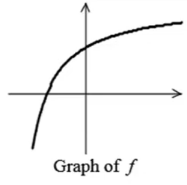
\includegraphics[width=0.3\textwidth]{9.1.1.PNG}
    \end{center}

    $P_2(x)=f(0)+f'(0)x+\frac{f''(0)}{2!}x^2$.

    We have $f''(0)=2c$

    $f(0)=a>0$, so above $x$-axis.

    $f'(0)=b>0$ means that $f(x)$ is increasing.

    $f''(0)=2c<0$ so $f(x)$ is concave down.
\end{example}

\begin{example}
    Suppose that the function $f(x)$ is approximated near $x=4$ by a third-degree Taylor polynomial $P_3(x)=2-5(x-4)^2+8(x-4)^3$.

    (a) Find the value of $f(4), f'(4), f''(4)$, and $f'''(4)$.

    $f(4)=2, f'(4)=0, f''(4)=-10, f'''(4)=48$.

    (b) Does $f$ have a local maximum, a local minimum, or neither at $x=4$? Justify your answer.

    $f$ must have a critical point at $x=4$. Since $f'(4)=0$ and $f''(4)=-10<0$, $f$ has a local maximum at $x=4$.
\end{example}

\ex The Taylor series about $x=2$ for a certain function $f$ converges to $f(x)$ for all $x$ in the interval of convergence. The nth derivative of $f$ at $x=2$ is given by $f^{(n)}(2)=\frac{(n+1)!}{3^n}$ for $n\geq 1$ and $f(2)=1$. Write the third-degree Taylor polynomial for $f$ about $x=2$.

\section{Radius and Interval of Convergence}
An infinite series such as $\sum_{n=1}^{\infty} \frac{5^n}{n!}$ is called a series of constants. Each term of the series is a constant.

An infinite series such as $\sum_{n=1}^{\infty} \frac{(x-5)^n}{n!}$ is called a power series, centered at $x=5$. Each term of the series contains a power of $x-5$.

\begin{definition}
    If $x$ is a variable, then an infinite series of the form 
    \[ \sum_{n=0}^{\infty}a_n(x-c)^n = a_0+a_1(x-c)+a_2(x-c)^2+\dots+a_n(x-c)^n + \dots \]
    is called a power series centered at $c$, where $c$ is a constant.
\end{definition}

A power series in $x$ can be viewed as a function of $x$, $f(x)=\sum_{n=0}^{\infty}a_n (x-c)^n$, where the domain of $f$ is the set of all $x$ for which the power series converges. We will be finding the domain of the power series in this section. Each power series converges at its center $c$.

For a power series centered at $c$, there are three possibilities:
\begin{enumerate}
    \item The series converges only at $c$.
    \item There exists a real number $R>0$ such that the series converges for $|x-c|<R$ and diverges for $|x-c|>R$.
    \item The series converges for all real numbers.
\end{enumerate}

The number $R$ is the radius of convergence of the power series.

If the series converges only at $c$, the radius of convergence is $R=0$.

If the series converges for all $x$, the radius of convergence is $R=\infty$.

The set of all values of $x$ for which the power series converges is the interval of convergence of the power series.

The Ratio Test is used to find the radius and interval of convergence. The Ratio Test says that a series will converge if $\lim_{n\to\infty}\left|\frac{a_{n+1}}{a_n}\right|<1$ so we will find the $\lim_{n\to\infty}\left|\frac{a_{n+1}}{a_n}\right|$ and then determine the value(s) of $x$ for which the limit is less than 1.

\pagebreak
\begin{example}
    Find the radius of convergence and the interval of convergence. Be sure to check the endpoints. (Note: Every time you are asked to find the interval of convergence, you must check to see if the endpoints are included in the interval.)
    \[ \sum_{n=1}^{\infty} \frac{(-1)^{n+1}(x-5)^n}{n2^n} \]

    Simplifying the inside of the summation gives us $\lim_{n\to\infty} \left| \frac{x-5}{2}\right|<1$.

    The radius of convergence is therefore $2$ because we get $|x-5|<2$.

    Now solving for $x$ gives $3<x<7$.

    Now check the endpoints.

    $x=3$ will give a harmonic series so it diverges. $x=7$ will give $\sum_{n=1}^{\infty}\frac{(-1)^{n+1}}{n}$ which converges.

    Therefore the interval of convergence is $3<x\leq 7$.
\end{example}

\ex Find the radius of convergence and the interval of convergence. $\sum_{n=0}^{\infty}\frac{(-1)^n x^{2n+1}}{(2n+1)!}$

\ex Find the radius of convergence and the interval of convergence. $\sum_{n=1}^{\infty}n!(x-3)^n$


\section{Taylor Series}
Previously we learnt how to find a Taylor polynomial for a function $f$. Now we will find a Taylor series for a function $f$.

The Taylor Series centered at $x=c$ is given by 
\[ f(c)+f'(c)(x-c)+\frac{f''(c)}{2!}(x-c)^2 + \dots + \frac{f^{(n)}(c)}{n!}(x-c)^n + \dots = \sum_{n=0}^{\infty}\frac{f^{(n)}(c)}{n!}(x-c)^n \]

If $c=0$, the series is called a Maclaurin series.

\begin{example}
    Find a Taylor series for $f(x)=e^{5x}$ centered at $c=2$. Give the first four nonzero terms and the general term.

    $f(x)=e^{5x}, f'(x)=5e^{5x}, f''(x)=25e^{5x}, f'''(x)=125e^{5x}$.

    $f(2)=e^{10}, f'(2)=5e^{10}, f''(2)=25e^{10}, f'''(x)=125e^{10}$.

    so we get 
    \[ e^{10}+5e^{10}(x-2)+\frac{25e^{10}}{2!}(x-2)^2 + \frac{125e^{10}}{3!}(x-2)^3 + \dots + \sum_{n=0}^{\infty}\frac{e^{10}5^n(x-2)^n}{n!}=e^{5x} \]
\end{example}

There are three special Maclaurin series you must know. These are the series for $e^x$, $\sin x$, and $\cos x$.

To derive a series for $e^x$:
\[ e^x=1+x+\frac{x^2}{2!}+\frac{x^3}{3!} \]

For what values of $x$ does $e^x$ equal the series that you found?
\begin{center}
    $e^x = \sum_{n=0}^{\infty} \frac{x^n}{n!}$ for $-\infty<x<\infty$
\end{center}

To derive a series for $\sin x$:
\[ \sin x=x-\frac{x^3}{3!}+\frac{x^5}{5!}-\dots \]

For what values of $x$ does $\sin x$ equal the series that you found?
\begin{center}
    $\sin x = \sum_{n=0}^{\infty}\frac{(-1)^n x^{2n+1}}{(2n+1)!}$ for $-\infty<x<\infty$
\end{center}

To derive a series for $\cos x$:
\[ \cos x = 1-\frac{x^2}{2!}+\frac{x^4}{4!}-\dots \]
\begin{center}
    $\cos x = \sum_{n=0}^{\infty} \frac{(-1)^n x^{2n}}{(2n)!}$ for $-\infty<x<\infty$
\end{center}

We can manipulate these three special series (or any series we are given) to find other series by using the techniques, called manipulation techniques. These include:
\begin{enumerate}
    \item Substituting into the series 
    \item Multiplying or dividing the series by a constant and/or a variable 
    \item Adding or subtracting two series 
    \item Differentiating or integrating a series 
\end{enumerate}

\begin{example}
    Find a Maclaurin series for $f(x)=\sin(x^2)$. Find the first four nonzero terms and the general term.

    We previously found the series for $\sin x$, so we just square everything to get 
    \[ \sin(x^2)=x^2-\frac{x^6}{3!}+\frac{x^{10}}{5!}-\frac{x^{14}}{7!}+\dots \sum_{n=0}^{\infty}\frac{(-1)^n x^{4n+2}}{(2n+1)!} \]
\end{example}

\ex Find a Maclaurin series for $f(x)=x\cos x$. Find the first four nonzero terms and the general term.

\ex Find a Maclaurin series for $h(x)=\frac{e^x+e^{-x}}{2}$. Find the first four nonzero terms and the general term.

\begin{example}
    (a) Find a Maclaurin series for $f(x)=e^x$. Give the first four nonzero terms and the general term.

    We know this is $e^x=1+x+\frac{x^2}{2!}+\frac{x^3}{3!}+\dots \frac{x^n}{n!}$

    (b) Use your answer to (a) to find $\lim_{x\to 0} \frac{f(x)-1}{2x}$

    This is $\lim_{x\to 0}\frac{(1+x+\frac{x^2}{2!}+\frac{x^3}{3!}+\dots)-1}{2x}$.

    This limit comes out to $\frac{1}{2}$.
\end{example}

\ex (a) Find a Maclaurin series for $f(x)=\cos x$. Give the first four nonzero terms and the general term.

(b) Use your answer to (a) to find a Maclaurin series for $g(x)=\frac{1-\cos x}{x^2}$. Give the first four nonzero terms and the general term.

(c) Use your answer in (b) to approximate the value of $\int_0^1 \frac{1-\cos t}{t^2}dt$ so that the error in your approximation is less than $\frac{1}{500}$. Justify your answer.

\pagebreak
\begin{example}
    Find a power series for $f(x)=\frac{1}{1-x^2}$, centered at $x=0$. Give the first four nonzero terms and the general term. What values of $x$ does your series converge to $f(x)$?

    In this, $a=1$ and $r=x^2$. We have $1+x^2+x^4+x^6+\dots (x^2)^n = x^{2n}$.

    We have $|x^2|<1$, so $-1<x<1$ and this never converges at its endpoints.
\end{example}

\ex Find a power series for $f(x)=\frac{1}{4+x}$ centered at $x=0$. Give the first four nonzero terms and the general term. For what values of $x$ does your series converge to $f(x)$?

\ex Find a power series for $f(x)=\frac{15}{2x-1}$ centered at $x=2$. Give the first four nonzero terms and the general term. For what values of $x$ does your series converge to $f(x)$?

\begin{example}
    Find the sum of $1+\frac{3}{1!}+\frac{9}{2!}+\frac{27}{3!}+\dots+\frac{3^n}{n!}+\dots$

    Note this looks like $e^x$ series expansion. This is actually the sum $\sum_{n=0}^{\infty}\frac{3^n}{n!}=e^3$.
\end{example}

\ex Find the sum of $2-\frac{8}{3!}+\frac{32}{5!}-\frac{128}{7!}+\dots+\frac{(-1)^n 2^{2n+1}}{(2n+1)!} + \dots $

\ex Find the sum of $1-\frac{2}{3}+\frac{4}{9}-\frac{8}{27}+\dots + \left(-\frac{2}{3}\right)^n + \dots$

\begin{theorem}
    If the function given by 
    \[ f(x)=a_0+a_1(x-c)+a_2(x-c)^2+a_3(x-c)^3+\dots = \sum_{n=0}^{\infty}a_n(x-c)^n \]
    has a radius of convergence of $R>0$, then on the interval $(c-R, c+R)$, $f$ is differentiable (and therefore continuous). Moreover, the derivative and antiderivative of $f$ are as follows:
    \[ f'(x)=a_1+2a_2(x-c)+3a_3(x-c)^2 + 4a_4 (x-c)^3\dots = \sum_{n=1}^{\infty}na_n(x-c)^{n-1}\]
    \[ \int f(x)dx = C+a_0(x-c)+\frac{a_1(x-c)^2}{2}+\frac{a_2(x-c)^3}{3}+\dots = C+\sum_{n=0}^{\infty}\frac{a_n(x-c)^{n+1}}{n+1} \]

    The radius of convergence of the series obtained by differentiating or integrating a power series is the same as that of the original power series. The interval of convergence, however, may differ as a result of the behavior of the endpoints.
\end{theorem}

\pagebreak
\begin{example}
    The function $f$ is defined by $f(x)=\frac{1}{1-x}$.

    (a) Write the Maclaurin series for $f$. Give the first four nonzero terms and the general term. For what values of $x$ does the series converge.

    $1+x+x^2+x^3+\dots x^n$ for $-1<x<1$

    (b) Use your answer to (a) to find the Maclaurin series for $f'(x)$. Give the first four nonzero terms and the general term. For what values of $x$ does the series converge?

    $f'(x)=1+2x+3x^2+4x^3+\dots nx^{n-1}$. Converges at $-1<x<1$.

    $f'(x)=\sum_{n=1}^{\infty}nx^{n-1}$

    (c) Use your answer in (b) to find the sum of the infinite series 
    \[ 1+\frac{2}{3}+\frac{3}{9}+\frac{4}{27}+\dots + \frac{n}{3^{n-1}} \]

    This is geometric $\sum \frac{n}{3^{n-1}}\implies \sum n\left(n\frac{1}{3}\right)^{n-1}=\frac{9}{4} $

    (d) Use your answer in (a) to find the Maclaurin series for $\int_0^x f(t)dt$. Give the first four nonzero terms and the general term. For what values of $x$ does the series converge?

    The integral is $x+\frac{x^2}{2}+\frac{x^3}{3}+\frac{x^4}{4}+\dots \frac{x^{n+1}}{n+1}$.

    The endpoints end up being $-1\leq x<1$.
\end{example}

\ex (e) Use your answer to (d) to find the sum of the infinite series 
\[ \frac{1}{3}+\frac{1}{3^2\cdot 2}+\frac{1}{3^3\cdot 3}+\frac{1}{3^4\cdot 4}+\dots + \frac{1}{3^{n+1}\cdot (n+1)}+\dots \]

\section{Lagrange Error Bound}
Given: $f(x)$ = power series in $x$.

A partial sum is the first ``few'' terms of the series.

The tail is the rest of the terms of the series after a partial sum.

The remainder is the number you get by ``adding'' all the terms in the tail.

So $f(x)$ = partial sum $+$ remainder 

The error is the error you make by assuming $f(x)$ = the partial sum. So the error is the same number as the remainder. An error bound is a number 
known to be greater than the absolute value of the remainder.

For an alternating series, the absolute value of the first term of the tail is an error bound.

In the integral test for convergence, the improper integral is an error boudn.

Now, consider what Monsieur Lagrange is credited with showing. The Lagrange Remainder (the error) is exactly equal to the first term of the tail, but with its derivative evaluated at $x=c$ (about which the series is expanded) but at some number $z$ which is between $c$ and the value of $x$ at which you are evaluating the function. As this value of $z$ comes from (repeated) application of the mean value theorem, there is often no way of knowing exactly what $z$ equals.
But if you can find a number that is an upper bound for the derivative between $c$ and $x$, then you can find a Lagrange Error Bound.

Recall the Taylor Theorem from above.

\pagebreak
\begin{example}
    The function $f$ has derivatives of all orders for all real numbers $x$. Assume that $f(2)=6, f'(2)=4$, $f''(2)=-7$, $f'''(2)=8$.

    (a) Write the third-degree Taylor polynomial for $f$ about $x=2$, and use it to approximate $f(2.3)$. Give three decimal places.

    Answer: 6.921
    
    (b) The fourth derivative of $f$ satisfies the inequality $|f^{(4)}(x)|\leq 9$ for all $x$ in the closed interval $[2,2.3]$. Use this information to find a bound for the error in the approximation of $f(2.3)$ found in part (a).

    error$\leq \left| \frac{(2.3-2)^4}{4!}\right| \leq 0.0030375$

    (c) Use your answers in parts (a) and (b) to find an interval $[a,b]$ such that $a\leq f(2.3)\leq b$. Give three decimal places.

    $6.918\leq f(2.3)\leq 6.924$
\end{example}

\ex Let $f$ be the function given by $f(x)=\sin\left(5x+\frac{\pi}{3}\right)$ and let $P(x)$ be the third-degree Taylor polynomial for $f$ about $x=0$. 

(a) Find $P(x)$.

(b) Use the Lagrange error bound to show that $\left| f\left(\frac{1}{15}\right)-P\left(\frac{1}{15}\right)\right|<\frac{1}{1200}$.

\section{More on Error}
Alternating Series Remainder 

If a series has terms that are alternating, decreasing in magnitude, an dhaving a limit of 0, then the series converges so that it has a sum $S$. If the sum $S$ is approximated by the nth partial sum, $S_n$, then the error in the approximation, $|R_n|$ which equals $|S-S_n|$, will be less than the absolute value of the first omitted or truncated term, $a_{n+1}$.

In other words, if the three conditions are met, you can approximate the sum of the series by using the nth partial sum, $S_n$, and your error will be bounded by the absolute value of the first truncated term, $a_{n+1}$.

\begin{example}
    The Taylor series about $x=2$ for a certain function $f$ converges to $f(x)$ for all $x$ in the interval of convergence. The nth derivative of $f$ at $x=2$ is given $f^{(n)}(2)=\frac{(-1)^n}{3^n}$ and $f(2)=\frac{1}{3}$. 

    (a) Write the second-degree Taylor polynomial for $f$ about $x=2$.

    $P_2(x)=\frac{1}{3}-\frac{1}{3}(x-2)+\frac{\frac{1}{9}}{2!}(x-2)^2$

    (b) Show that the second-degree Taylor polynomial for $f$ about $x=2$ approximates $f(3)$ with an error less than 0.01.

    $f(3)\approx \frac{1}{18}$.

    error $<\frac{1}{162}$ which is less than $\frac{1}{100}$ 
\end{example}
\end{document}